%!TEX encoding = UTF-8 Unicode
%!TEX root = ../compendium.tex

\Lab{\LabWeekNINE}

\begin{Goals}
\item Kunna skapa och använda matriser.
\item Kunna iterera över matriser med nästlade for-loopar.
\item Kunna använda sig av och förstå arv.
\item Förstå och träna på olika villkor med if-satser.
\item Känna till algoritmer för att lösa problem så som att ta sig igenom en labyrint eller slumpmässigt skapa en labyrint.
\end{Goals}

\begin{Preparations}
\item Gör veckans övningsuppgifter.
\item Läs om matriser i Scala-boken på sida (??).
\item Läs om arv i Scala-boken på sida (??).
\item Läs om olika algoritmer för att ta sig igenom en labyrint: \url{https://en.wikipedia.org/wiki/Maze\_solving\_algorithm}
\item (Frivillig) Läs om olika algoritmer för att skapa en slumpmässig labyrint: \url{https://en.wikipedia.org/wiki/Maze\_generation\_algorithm}.
\end{Preparations}

\subsection{Bakgrund}

I denna laboration kommer du att få rita labyrinter och sedan implementera en algoritm för att ta dig igenom dessa. En labyrint är ett rum som har en ingång och en utgång. Ingången är i de här fallen alltid längst ner i labyrinten, och utgången högst upp. Alla väggar är också parallella med antingen x-axeln eller y-axeln. Ett sätt att beskriva en sådan labyrint i kod är med hjälp av en matris av Boolean-element. Varje element i matrisen motsvarar då en ruta i labyrinten. Värdet \texttt{true} i matrisen representerar att det finns en vägg på motsvarande ruta i labyrinten och \texttt{false} representerar att där istället är en väg att gå på.

\begin{figure}[h]
	\begin{center}
		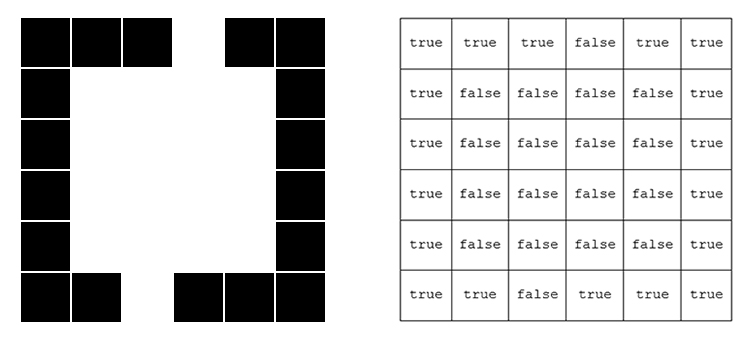
\includegraphics[width=0.7\textwidth]{../img/w09-lab/MazeAndMatrix.jpg}
	\end{center}
	\caption{Exempel på en matris-representation av en labyrint.}
\end{figure}

Det finns många olika sätt att ta sig igenom en labyrint men ett av de vanligaste sätten är att hålla vänster hand i vänster vägg och följa väggen med handen tills man når slutet av labyrinten. Detta fungerar för alla labyrinter där väggarna från ingången till utgången är sammankopplade. När man går igenom labyrinten finns det fyra olika riktningar att välja mellan som alla beskrivs i antal grader räknat från x-axeln, där höger motsvaras av 0 grader, uppåt motsvaras av 90 grader, vänster av 180 grader och nedåt av 270 grader.

% lägg till bild som visar hur man går runt ett hörn typ??

I den här laborationen kommer du använda dig av en färdig klass \texttt{Maze} som representerar en labyrint med hjälp av en Boolean-matris. Klassen har följande specifikation:

\begin{ScalaSpec}{Maze}
/**
 *  A class representing a maze.
 */
case class Maze(data: Vector[Vector[Boolean]]) {
  
  /**
   *  Returns a corresponding char from a boolean.
   *  @param b	The boolean which to convert to a char
   */
  def boolToChar(b: Boolean): Char

  /**
   *  Returns a String representation of the maze.
   */
  override def toString: Unit

  /**
   *  Checks if the coordinates x, y is inside the maze and if 
   so returns true, otherwise false.
   *  @param x		The x coordinate
   *  @param y		The y coordinate
   */
  private def insideMaze(x: Int, y: Int): Boolean

  /**
   *  Returns the x coordinate of the entry of the maze.
   */
  def getXEntry(): Int

  /**
   * Returns the y coordinate of the entry of the maze.
   */
  def getYEntry(): Int

  /**
   *  Checks if there is a wall left of the coordinates x, y at 
   given direction and if so returns true, otherwise false.
   *  @param direction	The direction of the turtle
   *  @param x					The x coordinate
   *  @param y					The y coordinate
   */
  def wallAtLeft(direction: Int, x: Int, y: Int): Boolean

  /**
   *  Checks if there is a wall in front of the coordinates x, y at 
   given direction and if so returns true, otherwise false.
   *  @param direction	The direction of the turtle
   *  @param x					The x coordinate
   *  @param y					The y coordinate
   */
  def wallInFront(direction: Int, x: Int, y: Int): Boolean

  /**
   *  Checks it the coordinates x, y is at the exit of the maze.
   *  @param x					The x coordinate
   *  @param y					The y coordinate
   */
  def atExit(x: Int, y: Int): Boolean

  /**
   *  Goes through the the maze and for every spot that is a wall 
   draws a brick of size blockSize in SimpleWindow.
   *  @param w		The window in which to draw the maze
   */
  def draw(w: SimpleWindow): Unit = ???
}

/**
 *  An object representing a maze.
 */
object Maze {

  /**
   *  Returns a Maze from a vector of Strings.
   *  @param xs	The vector of Strings that represent the maze
   */
  def fromStrings(xs: Vector[String]): Maze

  /**
   *  Returns a Maze from a specified file.
   *  @param fileName	   The name of the file that represent the maze
   */
  def fromFile(fileName: String): Maze

  /**
   *  Returns a Maze from a sequence of Strings.
   *  @param rows	The sequence of Strings that represent the maze
   */
  def apply(rows: String*): Maze

  /**
   *  Creates and returns a random maze.
   *  @param rows		The number of rows for the maze
   *  @param cols		The number of columns for the maze
   */
  def random(rows: Int, cols: Int): Maze = ???
}

\end{ScalaSpec}

\subsubsection{Den frivilliga uppgiften}

I den frivilliga uppgiften ska en slumpmässig labyrint genereras. Det finns flera olika algoritmer för att göra detta men den vi kommer använda här är en slumpmässig variant av Prims algoritm. Du kan läsa mer under \url{https://en.wikipedia.org/wiki/Maze\_generation\_algorithm} (De representerar en labyrint på ett annat sätt än vi gör i den här uppgiften vilket innebär att det inte kommer att se precis likadant ut).


\subsection{Obligatoriska uppgifter}

\Task I den här uppgiften ska du implementera en metod som ritar upp en labyrint i \texttt{SimpleWindow}.

\Subtask Läs igenom klassen och kompanjonsobjektet \texttt{Maze} och se till att du förstår det mesta. Du behöver inte förstå allt, men ju mer du förstår desto bättre och roligare, fråga om det är något som du tycker är oklart. Vad objektet \texttt{Maze} gör är att den tar in rader med strängar, antingen direkt som argument eller genom att läsa in från en fil. Utifrån detta skapar den sedan en Boolean-matris representation av labyrinten och skickar in som argument till \texttt{Maze}-klassen, där tecknet '\#' i en sträng representerar en bit av en vägg medan blanksteg representerar en bit av en gång.

\Subtask Du ska nu implementera metoden \texttt{draw} i klassen \texttt{Maze} som kommer att rita upp labyrinten i \texttt{SimpleWindow}. För att göra detta behöver du gå igenom matrisen \texttt{data} och undersöka elementen på varje plats. Om elementet på en viss plats är \texttt{true} ska det ritas upp en bit av en vägg på motsvarande plats i \texttt{SimpleWindow}. Detta kan du göra med hjälp av den färdigskrivna metoden \texttt{brickInTheWall}. Om elementet på en viss plats är \texttt{false} ska ingenting ritas upp.


\Task I den här uppgiften ska du skapa en klass med en main-metod som anropar din metod för att rita upp en labyrint.

\Subtask Skapa en ny klass \texttt{AMazeIngRace} genom att välja File -> New -> Scala Class. I denna klass ska du skriva en main-metod där du skapar ett objekt av \texttt{Maze} genom att läsa in från en fil (börja exempelvis med filen \texttt{maze1.txt}). Du måste även skapa ett objekt av \texttt{SimpleWindow} för att kunna skicka med när du anropar metoden \texttt{draw}. Anropa nu metoden \texttt{draw} på \texttt{Maze}-objektet och kontrollera att labyrinten ritas upp som den ska. Gör samma sak för resterande av filerna \texttt{maze2.txt}-\texttt{maze4.txt}, alla ska kunna ritas upp korrekt.

\Subtask Testa att rita en egen labyrint genom att skapa en textfil \texttt{maze5.txt} och lägg i samma mapp som övriga maze-filer. Kontrollera så att även denna labyrint ritas upp som den ska, och fixa annars till metoden \texttt{draw} så att den fungerar som tänkt. Observera att din labyrint inte alls behöver vara avancerad, det är inte meningen att den här uppgiften ska ta lång tid utan är till för att du ska få pröva på att rita en egen labyrint och se den förverkligas i din main-klass.


\Task I den här uppgiften ska du implementera en algoritm för att få en sköldpadda att ta sig genom en labyrint genom att alltid hålla i väggen med vänster hand (eller kanske fot i det här fallet). För detta ska du skapa en ny klass \texttt{MazeTurtle} som ska ha följande uppbyggnad:

\begin{ScalaSpec}{MazeTurtle}
/**
 * A Turtle that can walk through a maze with a specified color.
 * @param window     The window the turtle should be placed in.
 * @param position   A Point representing the turtle's starting coordinates.
 * @param angle      The angle between the turtle direction and the X-axis 
 measured in degrees.
 * @param isPenDown  A boolean representing the turtle's pen position. 
 True if the pen is down.
 * @param color		   The color with which the turtle will walk.
 * @param maze	     The maze in which the turtle will walk.
 */
class MazeTurtle(window: SimpleWindow, private var position: Point, 
private var angle: Double, private var isPenDown: Boolean, 
color: Color, maze: Maze) extends ColorTurtle(window, position, angle, 
isPenDown, color) {

  /**
   * Lets the turtle walk through the maze from entry to exit by 
   following the wall to left side of the turtle.
   */
  def walk(): Unit = ???
}

\end{ScalaSpec}

\Subtask Skapa en ny klass \texttt{MazeTurtle} som ärver från klassen \texttt{ColorTurtle}. \texttt{MazeTurtle} ska ta in ett extra argument, nämligen ett av typen \texttt{Maze} som representerar den labyrint som sköldpaddan ska gå i. Observera att du här behöver importera klasserna \texttt{Turtle} och \texttt{ColorTurtle} från en tidigare laboration. Detta gör du genom att högerklicka på projektet, välj Build Path -> Configure Build Path, välj fliken Projects, klicka på Add... och markera rätt laboration och klicka slutligen på OK.

\Subtask Lägg till och implementera metoden \texttt{walk} i \texttt{MazeTurtle}. I metoden ska sköldpaddan med hjälp av tekniken att alltid hålla vänster hand i väggen ta sig genom labyrinten \texttt{Maze}, från början till slut. Varje steg motsvarar att flytta sig från en ruta till en annan i Boolean-matrisen i \texttt{Maze}. Sköldpaddan kommer alltså ta sig fram i labyrinten genom att undersöka för varje steg om den borde svänga vänster, gå rakt fram eller svänga höger beroende på hur den står i förhållande till vänster vägg. För att avgöra hur sköldpaddan ska gå kan den använda sig av metoderna \texttt{wallInFront} och \texttt{wallAtLeft} som finns i \texttt{Maze}.

\Subtask Lägg till kod i \texttt{AMazeIngRace} som skapar en sköldpadda av typ \texttt{MazeTurtle} och sedan låter denna gå igenom en labyrint med metoden \texttt{walk}. Testa att din \texttt{MazeTurtle} fungerar som den ska! Sköldpaddan ska klara att ta sig igenom alla labyrinter i filerna \texttt{maze1.txt}-\texttt{maze4.txt} samt labyrinten som du skapat själv.


\subsection{Frivillig extrauppgift}

Prims algoritm används för att koppla ihop alla punkter i en graf med så få antal kopplingar som möjligt. Tänk dig att varje punkt i en graf representerar en ruta i en labyrint och att en koppling motsvarar ställen där du kan gå i labyrinten, det vill säga två öppna rutor (rutor där det inte finns någon vägg och som du därmed kan gå på) intill varandra.

I praktiken fungerar algoritmen så att den väljer en slumpmässig ruta intill en redan öppen ruta och undersöker om det finns någon annan öppen ruta intill. Om så är fallet låter den rutan förbli en vägg annars öppnar den rutan (det vill säga gör om  rutan från en vägg till en gång). Detta upprepas tills dess att alla rutor har undersökts.

Eftersom det i vårat fall endast ska finnas en in- och utgång i labyrinten måste detta hanteras på ett lite annorlunda sätt.

\begin{enumerate}
	\item Börja med att slumpmässigt välja en av rutorna i nedersta raden och öppna den rutan samt rutan ovanför. Detta motsvarar ingången till labyrinten.
	\item Applicera nedanstående algoritm på alla rutor i labyrinten utom de rutor i ytterkanten av matrisen som utgör labyrintens vägg.
	\item Slutligen letar vi efter en slumpmässig ruta på näst översta raden som är öppen och öppnar rutan ovanför denna, vilket kommer bli utgången för labyrinten.
\end{enumerate}

\begin{figure}[h]
	\begin{center}
		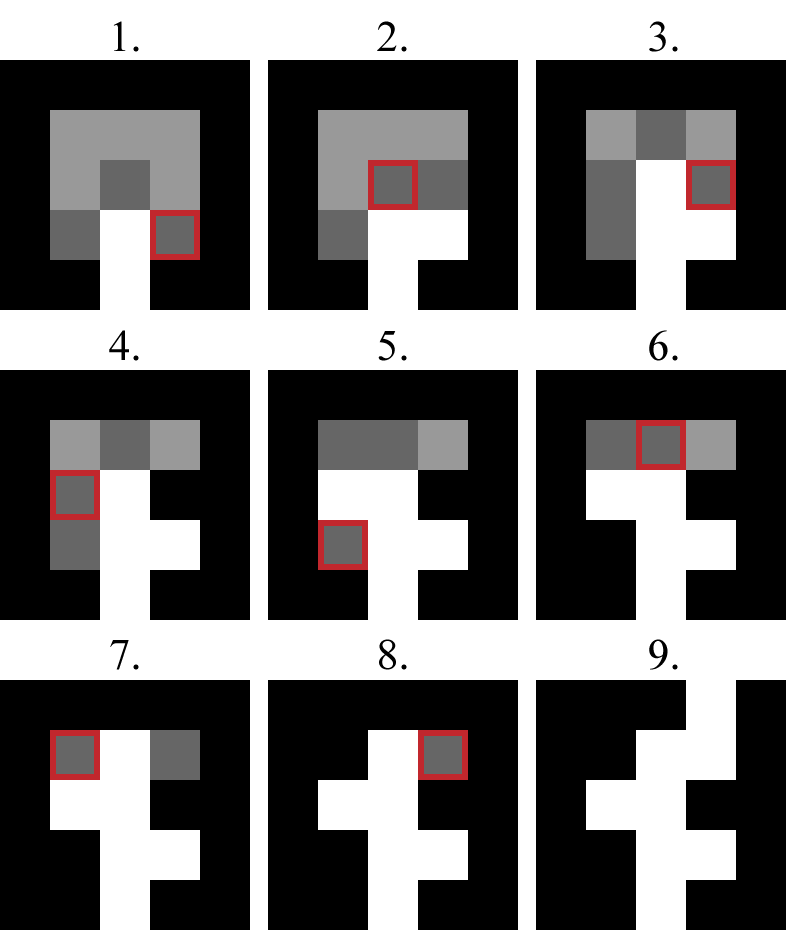
\includegraphics[width=0.45\textwidth]{../img/w09-lab/AlgorithmVisualized.png}
	\end{center}
	\caption{Visualisering av algoritmen när den genererar en labyrint av storleken 5x5.}
\end{figure}

\subsubsection{Psuedokod}
\begin{Code}
def random(rows, cols)
	labyrint = matris(rows, cols) med inga öppna rutor
	buffer = lista(koordinater till rutor)
	välj en slumpmässig ruta i nedersta raden och öppna den
	öppna rutan ovanför
	lägg till rutorna runt om till buffer
	while (buffer inte är tom)
		element = slumpmässigt element i buffer
		if (element har tre väggar intill sig)
			öppna rutan för de koordinater som element innehåller
			lägg till rutorna runt om element till buffer
		ta bort element från buffer
	hitta en ruta som är öppen i näst översta raden
	öppna rutan ovanför
\end{Code}


\Task I den här uppgiften ska du implementera en algoritm som skapar en slumpmässig labyrint.

\Subtask Inspektera ovanstående pseudokod och försök förstå den. Fråga gärna om något är oklart! Läs även de färdigskrivna metoderna \texttt{addWallToList} och \texttt{threeWallsAround} i metoden \texttt{random} i \texttt{Maze} och se om du kan förstå vad de gör.

\Subtask Implementera metoden \texttt{random} i \texttt{Maze} som skapar och returnerar en slumpmässigt utformad labyrint med hjälp av pseudokoden ovan (eller på egen hand för den modiga/nyfikna). Ta hjälp av metoderna \texttt{addWallToList} och \texttt{threeWallsAround}.

\Subtask Skapa en ny slumpmässig labyrint i \texttt{AMazeIngRace} genom att anropa metoden \texttt{random}. Ett bra värde att använda när du anropar metoden är något tal mellan 50 och 100. Det vill säga anropa metoden genom att exempelvis skriva \texttt{random(50, 50)}. När du har slumpat fram en labyrint, testa att låta din sköldpadda gå igenom labyrinten och se om den lyckas!

\begin{figure}[h]
	\begin{center}
		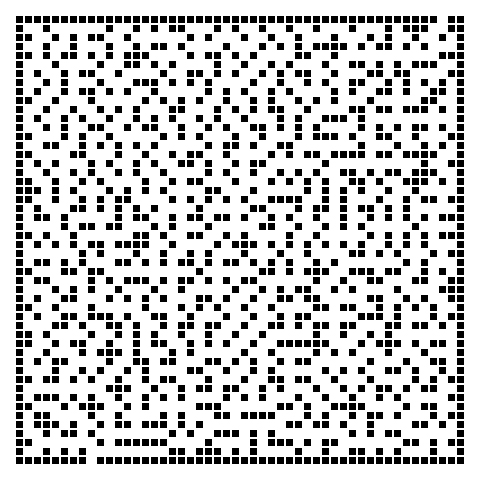
\includegraphics[width=0.3\textwidth]{../img/w09-lab/RandomMaze.jpg}
	\end{center}
	\caption{Ett exempel på hur en slumpmässigt utformad labyrint kan se ut.}
\end{figure}

